\documentclass[12pt]{article}
\usepackage[francais]{babel}
\usepackage[UTF8]{inputenc}
\usepackage[T1]{fontenc}
\usepackage{times}
\usepackage{helvet}
\usepackage{graphicx}
\usepackage{fancyhdr}
\usepackage{eurosym}
\usepackage{color}
\usepackage[tight]{shorttoc} 
\usepackage{soul}
\usepackage[ left = 4.5cm, right = 3.5cm]{geometry}

\renewcommand{\baselinestretch}{1.5}
\setlength{\parindent}{3cm}

\pagestyle{fancyplain} \chead{}\lhead{\textit{Les Professionnels}} \rhead{\emph{\textit{Evasion}}}

\definecolor{pseudorouge}{RGB}{200, 50, 50}
\definecolor{pseudoblue}{RGB}{20,10,230}
\definecolor{texteGris}{RGB}{50,50,75}

\begin{document}
\thispagestyle{empty}
\begin{center}
\fontsize{21}{21}{\textbf{Rapport de Soutenance 2 \vspace*{0.2cm}}}

\end{center}

\vspace*{0.7cm}

\begin{center}
\fontsize{21}{21}{\textbf{- Les Professionnels/}}
\fontsize{21}{21}{\textbf{2013-2014 -}}
\end{center}

\vspace*{0.5cm}

\begin{center}

\includegraphics[scale=01.0]{evasion}
\end{center}

\vspace*{0.5cm}

\fontsize{14}{14}
\begin{center}
{Lenny \textcolor{pseudorouge}{\textit{"Le Noob"}} Danino - danino\_l}
\end{center}
\begin{center}
Louis \textcolor{pseudoblue}{\textit{"El Parain"}} Kédémos - kedemo\_l
\end{center}
\begin{center}
Anatole \textcolor{pseudoblue}{\textit{"Totonut"}} Moreau - moreau\_a
\end{center}
\begin{center}
Khalis Chalabi - chalab\_k
\end{center}

\begin{center}

\includegraphics[scale=00.20]{infini}
\end{center}


\setlength{\headheight}{13pt} % Haut de page
\setlength{\headsep}{2.5cm} % Entre le haut de page et le texte
\setlength{\footskip}{2.5cm}



\setcounter{tocdepth}{1} 

\newpage
\thispagestyle{empty}
\pagestyle{fancyplain} \chead{}\lhead{\textit{Les Professionnels}} \rhead{\emph{\textit{Evasion}}}
\setcounter{tocdepth}{1} 
\tableofcontents


\newpage
\setcounter{page}{1} 


\section{Rappel du cahier des charges}

A notre entrée à EPITA, il nous a été demandé de réaliser un projet. Plus communément appelé \textit{Projet de sup}, il est à réaliser en C\# ou en Caml. Il s'agit de deux langages de programmations. Le C\# est un langage de programmation développé par Microsoft. Il est particulièrement adapté au développement d'applications destinées à Windows. Alors que Caml permet de développer pour un plus large panel de systèmes d'exploitations mais ne fourni aucun outil spécifique à un système d'exploitation. Pour ce projet, le sujet et la réalisation ont été laissés à notre libre choix. Nous avons décidé, comme beaucoup de nos camarades, de réaliser un jeu à l'aide du C\#.

Le jeu pourrait se définir comme un \textit{Prison Break Like}. Un individu doit s'échapper d'une prison sans être repéré. Une fois dehors, il devra récupéré de l'argent, des faux papiers, un moyen de transport pour pouvoir s'échapper du pays. Au cours de son périple, il pourra renconrer différents types d'ennemis, il pourra utiliser des objets, allant d'une simple clé à un pistolet.

Pour réaliser ce projet, le choix des langages a été imposé. Nous avions la possibilité de développer en C\# ou en Caml. Au vu de l'orientation de notre projet, nous avons immédiatement opté pour le C\#. Ce dernier propose tout les outils nécessaires à la réalisation d'un jeu vidéo. Un module a particulièrement retenu notre attention : XNA. XNA est un framework, ou un ensemble d'outils, destiné à la création de jeux vidéos pour Windows. Un jeu assez célèbre a été réalisé avec XNA, il s'agit de Forza, un jeu développé par Microsoft. 

De plus, nous souhaitions faire un jeu vidéo entièrement en 3D. XNA permet justement de faire du développement 3D, en proposant des outils beaucoup plus simple que ceux disponibles sur Internet.

Au début du jeu, nous voulions laissé la possibilité au joueur de choisir un personnage parmi d'autres, avec une certaine capacité. Ce personnage aurait aussi été capable de lancer des objets. Pour pouvoir s'infiltrer ou s'exfiltrer d'un lieu, ce même personnage aurait eu la capacité de marcher doucement, courir, s'accroupir ou d'ouvrir les portes. Pour ajouter une certaine compétition au jeu, nous avions en tête de réaliser un timer. Ainsi, les meilleurs temps réaliser par les joueurs pour s'échapper auraient pu être sauvegardés. Cela implique donc la création d'un site web et d'une interface réseau. Et enfin, pouvoir jouer en ligne en multijoueur a aussi été l'un de nos objectifs pour ce projet.

Malheureusement, à cause d'un problème de gestion du temps et d'une surestimation de nos capacités, certaines choses n'ont pas pu être réalisées. Mais beaucoup d'autres l'ont été. Nous avons réussi à faire un jeu en 3D. Cet aspect du développement a été le plus dur. Les personnages, le décors sont affichés en 3D. De plus, les personnages sont dotés seulement d'une animation de marche. Ils ne peuvent pas courir ou s'accroupir. En revanche, ils sont capables d'utiliser des armes comme un pistolet ou un couteau. L'aspect multijoueur a été plutôt bien développé. On peut en effet jouer en équipe en ligne ou en local sur un même ordinateur. L'interface réseau ayant été développée, il n'a pas été compliqué d'y ajouter un timer et d'enregistrer en ligne les temps réalisés par les joueurs. \\

Au début du projet, nous avons fait des prévisions de réalisation et un partage des tâches en fonction des capacités de chacun. Bien que certaines tâches n'aient pas été réalisées, le planning prévisionnel a été respecté. C'est à dire que les points que nous avons choisi de conserver ont progressé comme indiqué sur le planning. Nous avons aussi dû nous adapter pour la répartition du travail. Certains aspects étaient en réalité plus difficile que prévu. Ils ont donc été attribués à d'autres membres du groupe, ayant plus d'aisance en programmation. 
\newpage

\section{Louis Kédémos}

\subsection{Récapitulatif des deux soutenances}

\subsubsection{Première soutenance}

La réalisation de ce projet a fait appel à de la 3D. Nous voulions avoir un jeu en trois dimensions. D'un point de vue qualité, pour un jeu d'infiltration, cela nous a semblé être un point important. D'un point de vue technique, nous pourrions ainsi améliorer nos capacités en informatique. Je me suis proposé pour réaliser cet aspect du jeu vidéo. Ayant pu trouver une masse abondante d'exemples utilisant le module 3D de XNA, mon travail ne semblait pas difficile. Mais petit à petit, plus j'en découvrais sur la 3D, plus cela devenait incompréhensible. Beaucoup de notions sont utilisées qui m'étaient jusque là inconnues. 

La première étape pour faire un jeu en 3D est bien sûr d'avoir un modèle 3D. Un modèle 3D est un fichier contenant des informations, des coordonnées plus précisément, permettant de dessiner dans l'espace un objet ou une personne. J'ai utilisé le logiciel de modélisation 3D Blender. Ma première modélisation n'était pas esthétique. Son but était plutôt de me permettre de tester la 3D assez rapidement. Cette étape terminée, le plus dur restait à venir. Il me fallait maintenant réussir à afficher ce modèle à l'écran. Les exemples sur internet étaient complets mais j'étais dans l'incapacité de les comprendre. A chaque tentative, le début de jeu plantait ou bien le modèle ne s'affichait pas correctement. Finalement, une vidéo sur Youtube m'a permis dee comprendre en détail comment XNA permettait de gérer la 3D. Commença la phase de test. Le modèle affiché a été affiché, tourné, redimensionné de nombreuses fois pour pouvoir maitrîser les règles qui régissent la 3D. 

Comprendre le fonctionnement de la 3D avec XNA a été assez ardu et assez long. Concrètement, il n'y a aucune animation de faite. Seul un personnage en 3D s'affiche à l'écran et se translate dans l'espace, mais ses membres ne bougent pas. 

Ma part du travail pour cette première soutenance a été essentiellement la gestion de la 3D. Mais j'ai malgré tout pu participer aux autres éléments du jeu. Avec Anatole, nous avons construit un menu d'accueil. Je lui ai montré comment réalisé des boutons de différents aspects selon si la souris est sur le bouton ou non. Durant cette première phase de développement, j'ai pris soin à ce que nous gardions un projet bien organisé. Si nous voulons rajouter ou modifier quelque chose, c'est possible sans toucher au reste du projet. Ainsi chaque membre du groupe peut travailler de son côté sur la tâche qui lui incombe dans avoir à se préoccuper des autres.

\subsubsection{Deuxième soutenance}

Lors de la première soutenance, la création des personnages ou des murs en 3D demandait beaucoup de travail. Il devenait urgent de rendre la création 3D plus facile, pour permettre des phases de tests plus poussés le plus tot possible. J'ai donc créé des fichiers qui permettent l'instanciation, l'affichage et la manipulation des modèles 3D aisés. Le héros est maintenant dirigeable par le joueur. Il peut se déplacer dans les quatre directions, tourner sur lui même. Réaliser ces déplacements a été compliqué. Pour cela, il faut utiliser le produit matriciel. Malheureusement, je n'avais pas les connaissances requises en mathématique pour manipuler le produit matriciel. Ce dernier est en effet non commutatif. C'est à dire qu'il faut faire les multiplications dans un ordre précis. Je ne l'ai compris que longtemps après la première soutenance. Lors de la première soutenance, les déplacementss'effectuaient que selon les axes représentés par les flèches noires : 

\begin{figure}[h]
\begin{center}
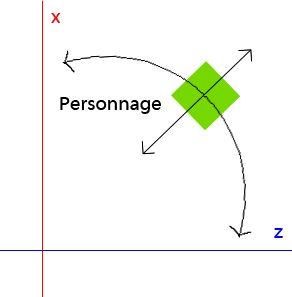
\includegraphics[scale=0.5]{deplac1.jpg}
\caption{Déplacements - première soutenance}
\end{center}
\end{figure}

Une fois le problème du produit matriciel compris et résolu, les déplacements ont pu se faire de façon plus précise : 

\begin{figure}[h]
\begin{center}
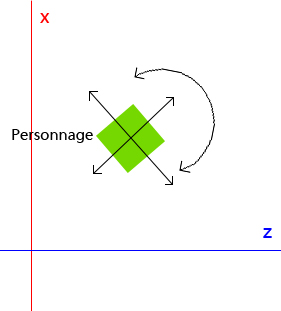
\includegraphics[scale=0.5]{deplac2.jpg}
\caption{Déplacements - deuxième soutenance}
\end{center}
\end{figure}

Après m'être occupé de l'affichage et du déplacement des modèles 3D, il a fallut m'occuper des collisions. Dans le monde du jeu vidéo, les collisions sont une des choses les plus importantes. Si les collisions sont mal gérées, lors d'un combat par exemple, on peut se faire tuer par l'ennemi sans avoir pu le toucher une seule fois. Je suis allé chercher des informations concernant les collisions sur internet. Les résultats ne manquaient pas. De nombreuses techniques sont expliquées. Je n'en ai retenu qu'une seule : celle utilisant des \bsc{Bounding Box}. Cette méthode définit une boîte virtuelle englobant chaque modèle 3D présent dans l'environnement. Ensuite une méthode de détection d'intersection permet de détecter si deux bouding boxe sont entrées en collisions. On peut voir un exemple de bounding box sur l'image suivant, elles apparaissent en trait blanc : 

\begin{figure}[h]
\begin{center}
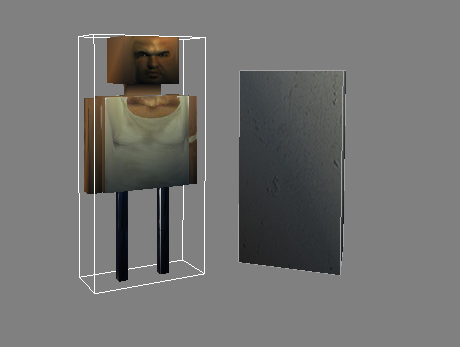
\includegraphics[scale=0.5]{BoundingBox.jpg}
\caption{Exemple de Bounding Box}
\end{center}
\end{figure}

Je n'ai pas eu le temps d'implémenter cette méthode pour la seconde soutenance. Des problèmes apparaissaient au fil du développement.



\subsection{Réalisations}

Pour cette troisième soutenance, nous n'avons pas eu assez de temps pour ajouter de nouvelles fonctionnalités à notre jeu. Nous avons dû en effet répartir notre énergie à nos partiels, nos cours et au projet. En conséquence, peu d'évolution majeures ont fait leurs apparitions entre la deuxième et la troisième soutenance. Dans la suite de cette partie, je détaille le travail que j'ai effectué, seul ou à plusieurs.

\subsubsection{Animations 3D}



Notre deuxième soutenance a vu l'apparition d'un générateur de carte et de l'affichage de carte. La gestion des différents éléments en 3D a aussi été rendue plus simple. Mais il manquait une chose essentielle : l'animation 3D. Les personnages 3D, lors de leurs déplacements, ne sont pas animés. Les jambes, les bras ne bougent pas. Les personnages sont simplement translatés dans l'espace. Ma première tâche a été de réaliser les animations des personnages. Une tâche ardue qui a requis de nombreuses heures de travail. Pour cela, j'ai utilisé le logiciel de modélisation 3D Blender. Il s'agit d'un logiciel libre assez simple qui permet une bonne introduction au graphisme 3D. L'animation des personnages se résume seulement à un pas complet. C'est à dire coordonner le mouvement de chaque membre du corps : l'avancement de chaque jambe et le contre-balancement des bras. Il suffit ensuite de jouer cette animation en boucle pour donner l'impression d'une marche. Chaque type de personnage à son type de marche. J'ai donc animer différement le personnage principale, les gardiens et les autres prisonniers. 

Pour l'affichage et le déplacement des modèles 3D, je me suis heurté à un premier problème. Il faut manipuler des matrices et le produit matricelle pour juste afficher un modèle. Malheureusement, je n'avais pas encore saisie la subtilité du produit matricielle : il n'est pas commutatif. J'ai perdu énormément de temps sur ce point au début. En ce qui concerne l'animation à proprement parler, j'ai rencontré une nouvelle difficulté. Pour la comprendre, il faut comprendre comment un modèle 3D est enregistré. Un modèle est en réalité un squelette sur lequel on vient poser une image, une texture comme on le ferait avec du papier peint. Et c'est ce squelette qui est enregistré en mémoire. Chaque mouvement ou rotation de chaque os de ce squelette est aussi enregistrée pour constituer plus tard une animation 3D. Pour animer le modèle, il faut dire au programme de charger l'état suivant du squelette. Mon problème a été justement de charger la position suivante. Je ne savais pas quelle propriété du modèle utiliser, ou comment faire pour modifier l'état du squelette. \\
Très peu de documentation existe sur Internet. Je n'ai réussi à trouver qu'un exemple issue du site officiel de microsoft. Mais cet exemple n'avait aucune explication ou commentaire. Déchiffrer les lignes de code a été assez ardu. Au fait de mon manque d'expérience en programmation 3D, beaucoup de temps a été nécessaire pour reproduire l'exemple. Une erreur revenait souvent : la même image était chargée sans arrêt. Après de nombreux tests infructueux, j'ai finalement réussi à obtenir une animation complète des personnages.

\newpage

\subsubsection{Création d'une intelligence artificelle}

A ce stade du développement, notre personnage est capable de se déplacer dans son environnement 3D et d'entrer en collision avec les murs, grâce au travail d'Anatole. Faire se déplacer les ennemis a donc été l'étape suivante dans le développement du jeu. La difficulté est de déterminé un chemin aléatoire dans la carte. Il faut que ce chemin soit libre de murs et d'ennemis, pour que le déplacement s'effectue sans encombre. Une fois ce chemin déterminé, il faut trouver un moyen de le faire parcourir par l'ennemi. Pour choisir un chemin aléatoire, nous définissons en premier lieu une distance maximale. Puis nous placons un marqueur à la position de départ de l'ennemi. Ensuite, une direction est choisie au hasard. Le programme suit ensuite cette direction jusqu'à l'intersection suivante, où il choisie une nouvelle direction au hasard. Ce processus est répété tant que la distance maximale n'est pas atteinte. Cela permet d'obtenir un parcours pseudo-aléatoire. 

Vient ensuite le problème du déplacement des ennemis. Nous savons où ils doivent aller, mais nous ne savons pas comment. Etant donné que le déplacement des ennemis ne concernait pas vraiment la boucle de jeu principale, une seule idée nous est apparue, à Anatole et moi. Il s'agissait d'utiliser des processus en parallèle, ou des \bsc{Thread}. Un thread est un outil du \bsc{C\#} qui permet d'exécuter deux actions en parallèles, ou en tout cas en donne l'illusion. Un ordinateur, naturellement, ne peut effectuer qu'une seule chose à la fois. Ainsi les ennemis sont capables de se déplacer de façon aléatoire et autonome, sans ralentir l'exécution principale. 

Mais se déplacer selon un chemin prédéfini en permanence n'est pas très "intelligent" pour une intelligence artificielle. C'est pourquoi Anatole et moi avons implémenté une capacité repérage aux ennemis.  Lorsque notre personnage se situe à une faible distance d'un ennemi et que celui-ci regarde dans la direction du personnage, alors on considère que le personnage est repéré. Dès lors, l'ennemi va poursuivre le héros, jusqu'à la mort de l'un des deux ou si le héros arrive à échapper à la surveillance de l'ennemi. 




\subsubsection{Utilisation d'armes}

Notre jeu dispose maintenant d'ennemis capables de se déplacer et d'un personnage. Il nous manquait encore la possibilité d'utiliser des armes, telles qu'un pistolet ou un couteau. Etant donné que ce point est encore relatif à la 3D, je m'en suis occupé. La première étape a été de modéliser des armes en 3D, avec Blender. Khalis s'en est occupé. Pour qu'un personnage se saississe d'une arme et qu'elle vienne se placer dans sa main, il faut placer un marqueur. Ce marqueur se situe à l'emplacement de la main droite. J'ai donc dû modifier les modèles 3D pour qu'ils intègrent un tel marqueur. Je peux ainsi récupérer la position et l'orientation de la main et y placer l'arme.

Quant à l'utilisation des armes, il a fallu créer deux classes différentes. Une pour les armes dites de corps à corps et une pour celles à distance. Lorsque l'on utilise une arme de corps à corps, la classe correspondante va vérifier si un ennemi se trouve à proximité de l'arme et qu'il se trouve en face du personnage. Si ces conditions sont réunies, alors on considère que l'utilisation de l'arme est positive, c'est à dire qu'elle a touché un ennemi. Déterminer de quel ennemi il s'agit est ensuite simple. Il ne reste plus  alors qu'à lui retirer un certain nombre de point de vie. La difficulté de cette méthode se situe dans la détection d'un ennemi. 




\newpage

\subsection{Conclusion personnelles}

A mon entrée en première année à EPITA, j'étais excité de devoir réaliser un projet durant le second semestre. Et au terme de ce projet, je suis toujours autant excité d'avoir eu à le faire. 

Evidemment, ces six mois a vu de nombreux différends entre les quatre membres du groupe. Mais à tout moment nous gardions une bonne cohésion. Une désolidarisation du groupe aurait signifier l'échec du projet. De mon point de vue, ce projet avait pour but premier de nous apprendre à travailler en équipe et non de nous apprendre à mener à terme un projet. 

J'ai été nommé chef de projet en début d'année. Ce rôle incombe de nombreuses responsabilités. J'ai dû axer notre groupe sur un chemin de développement que chaque membre acceptait. Assez passionnant au début, cela devient vite frustrant quand on doit effectuer des choix. 

Pour résumer cette expérience, je dirais que ça a été un plus pour mon futur à EPITA. En tant que chef de projet et membre d'un groupe, ce semestre a été enrichissant.Au lieu de ne rencontrer que des portes ouvertes, nombreuses sont celles à être restées fermées. A chaque nouveau problème, il me fallait trouver un compromis, une solution qui satisfasse toute l'équipe. Et à chaque fois, mes prises de déscisions étaient plus rapide. Ayant le plus d'expérience, j'ai souvent plaidoyer en faveur de certaines idées, jugeant celles-ci réalisables ou non. A l'inverse, si nous n'avions rencontrés aucune difficultés, ce projet ne nous aurait pas été profitable. Durant nos années d'études, il y aura de plus en plus de contraintes. Aprrendre à les gérer assez tôt est important. Parmi ces contraites, j'entends aussi bien les divergences d'avis que les contraintes techniques imposées par un client. 

J'ai appris aussi que constituer un groupe de projet avec des amis ne signifie pas forcément une bonne réussite de projet. 

Je dois avouer que les moments précédents nos soutenances ont été mes préférés. Nous voir habillés en costumes, l'air professionnel m'a donné l'impression de soutenir un projet à un niveau plus professionnel. Il ne s'agit bien sûr que d'une impression, la réalité étant différente. Mais cette impression, brève en comparaison des six mois de stress et de travail, m'a conforté dans mon choix d'être ingénieur.

\newpage
\listoffigures

\end{document}
